\documentclass[12pt,a4paper]{article}
\usepackage[utf8]{inputenc}
\usepackage{amsmath}
\usepackage{amsfonts}
\usepackage{amssymb}
\usepackage[brazil]{babel}
\usepackage{indentfirst}
\usepackage{listings}
\usepackage{url}
\lstset{numbers=left, numberstyle=\tiny, stepnumber=1, numbersep=5pt}
\RequirePackage{graphicx}
\title{jQuery}
\usepackage[left=3cm,right=3cm,top=2cm,bottom=2cm]{geometry}

\begin{document}
\begin{titlepage}

\begin{center}
\begin{figure}[htb]
		
		\label{figura:LogoIF}
	
		\centering
		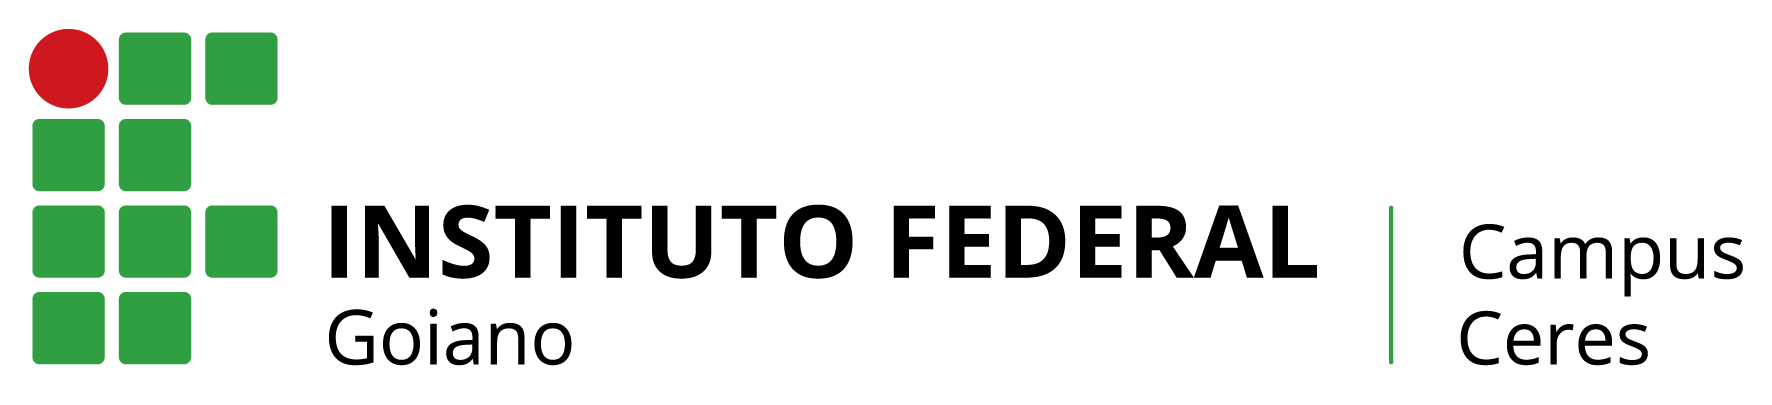
\includegraphics[width=6cm]{logo.png} 
\end{figure}


Instituto Federal Goiano - Campus Ceres\\
Bacharelado em Sistemas de Informação\\\vspace{8.0cm}

\textit{\textbf{\Large{EstatísticSI}}}\\\vspace{8.5cm}

Outubro\\
2017\\
\end{center}
\end{titlepage}

\tableofcontents

\newpage
\begin{center}
\textbf{\Large{EstatísticSI}}\\\vspace{0.5cm}
\end{center}
\section{Objetivo geral}%GGN

A ferramenta ``EstatísticSI"  surgiu do anseio de trabalhar o conteúdo de estatística com maior facilidade de interação, uso e aplicação, em prol da construção da ferramenta didática para apresentação na IV Gincana de Estatística promovida no Campus Ceres do IF Goiano, com intuito de posterior utilização em aulas da disciplina de Probabilidade e Estatística (e suas variantes) no Instituto Federal Goiano Campus Ceres.

\section{Características}%GGN

De acordo com a proposta, a ferramenta em questão aborda intrinsecamente o tema ``Estatística", oferecendo aplicabilidade, criatividade e inovação, que podem ser refletidas no quesito ensino-aprendizagem da disciplina citada. Trata-se de uma aplicação \textit{web}, promovendo portabilidade e facilidade de uso em qualquer lugar do mundo, desde que se tenha conexão à Internet. 

Para seu uso, o discente (ou usuário interessado) terá a possibilidade de utilização da ``EstatísticSI" para algumas das principais funções estatísticas, desde relações como média até testes ANOVA e Qui-Quadrado. Além disso, o acadêmico ainda terá a opção de salvar suas atividades, logando no sistema.
 
Ademais, para aqueles que querem entender como funcionam cada uma das atividades disponibilizadas, haverá uma sessão de ``drops", termo referente a vídeos curtos, capazes de ensinar os conceitos abordados e apresentados, oferecendo conhecimento interligado a ferramenta tecnológica. Os mesmos possuírão tradução na Língua Brasileira de Sinais (LIBRAS), garantindo maior acessibilidade.

\section{Funções estatísticas}

Para essa aplicação, selecionou-se as seguintes medidas e funções estatísticas. As mesmas foram agrupadas de acordo com grau de importância/estudo para os acadêmicos do 4$^{\circ}$ período do Curso de Bacharelado em Sistemas de Informação, levando em conta sua utilização na disciplina de Probabilidade e Estatística, ofertada na matriz curricular.

\begin{itemize}
\item \textbf{Tendência Central:} Medidas estatísticas as quais possuem valores que estão próximos do centro de um conjunto de dados. Tais relações estatísticas fazem parte do ramo da Estatística Descritiva.
	\begin{itemize}
		\item \textit{Média:} A média aritmética de um conjunto de dados equivale ao resultado da divisão decorrente da soma de todos os valores em questão pela quantidade de valores ou parcelas.
		\item \textit{Moda:} Trata-se do valor do conjunto que se repete com maior frequência.
		\item \textit{Mediana:} A mediana pode ser definida como o valor que se encontra no meio de um conjunto de dados, após ser ordenado crescentemente, tendo antes e depois de si a mesma quantidade de dados.
	\end{itemize}
\end{itemize}

\begin{itemize}
\item \textbf{Dispersão ou Variabilidade:} Parte da Estatística Descritiva, é o conjunto de medidas estatísticas capazes de medir as oscilações  de certa variável.
	\begin{itemize} 
		\item \textit{Amplitude:} Diferença entre o maior e menor valor de um determinado conjunto de dados.
		\item \textit{Variância:} É a média dos quadrados das diferenças dos valores em relação a sua média aritmética.
		\item \textit{Desvio Padrão:} Raiz quadrada das variâncias e representa quanto aquela medida pode variar.
		\item \textit{Coeficiente de Variação:} Valor expresso pela divisão do desvio padrão pela média, com dados expressos em porcentagem.
	\end{itemize}
\end{itemize}

\begin{itemize}
\item \textbf{Correlação:} Inerente a Estatística Inferencial, expressa quanto as variáveis resposta estão associadas entre si. Pode-se referir a força que mantém a união de dois conjuntos de valores.
	\begin{itemize} 
		\item \textit{Coeficiente de Correlação:} Medida capaz de assegurar a correlação entre variáveis resposta, sejam nulas, fracas, regulares ou fortes. O coeficiente também deve ser significativo.
		\item \textit{Coeficiente de Determinação:} Quadrado do coeficiente de correlação e refere-se a quanto uma variável pode influenciar no comportamento da outra.
	\end{itemize}
\end{itemize}

\begin{itemize}
\item \textbf{Regressão:} Análise para verificação de relação entre variável dependente e independente (variável resposta x tratamento).
	\begin{itemize} 
		\item \textit{Coeficiente de Determinação:} Medida também presente na regressão, pode inferir o quanto aquele modelo explica com mais exatidão a resposta em questão.
	\end{itemize}
\end{itemize}
		
\begin{itemize}
\item \textbf{Teste de Qui-quadrado:} Parte Inferencial, aliada a um teste não paramétrico, para avaliação de frequências. Usado para decidir se os valores observados se ajustam a uma determinada expectativa.
\end{itemize}

\begin{itemize}
\item \textbf{Teste F - ANOVA:} Teste paramétrico para análise de variância, responsável por estimativas de variância dado o quadrado médio. Por meio deste, verifica-se se de fato a variância é do tratamento ou apenas um possível erro.
\end{itemize}

\section{Referências}
\begin{enumerate}

\item COSTA, S. F. \textbf{Introdução Ilustrada à Estatística.} 4. ed. São Paulo: Harbra, 2005. 399 p.

\end{enumerate}

\end{document}